\subsection{Gestione di Progetto}
La responsabilità di gestione del progetto è attribuito al \textit{Responsabile di Progetto}. \\
Utilizzando tutti gli strumenti a disposizione il \textit{Responsabile di Progetto} avrà il compito di:
\begin{itemize}
	\item Pianificare le attività;
	\item Gestire le risorse;
	\item Analizzare e prevenire i rischi.
\end{itemize}

\subsubsection{Pianificazione delle attività}
Per pianificare le varie attività da svolgere il \textit{Responsabile di Progetto} dovrà utilizzare GanttProject per realizzare i diagrammi di Gantt.

\subsubsection{Coordinazione e gestione delle risorse}
Per gestire le risorse durante lo sviluppo del progetto, il \textit{Responsabile di Progetto} dovrà pianificare la quantità di ore che ogni risorsa dovrà dedicare a ciascuna attività.\\
Si è deciso di utilizzare il servizio di gestione dei \gls{task} e creazione di \gls{milestone} offerto da \gls{GitHub} spiegato nella sezione SEZIONE. Questo permette di accentrare le informazioni in un solo ambiente.

\subsubsection{Analisi e prevenzione dei rischi}
Durante l'avanzamento del progetto, il \textit{Responsabile di Progetto} deve monitorare costantemente il verificarsi dei rischi descritti nel \textit{Piano di Progetto v2.0.0}. La valutazione dei rischi deve essere aggiornata al mutare delle situazioni di pericolo, in occasione di significative modifiche al processo produttivo oppure all'introduzione di nuove tecnologie. Una volta completata la valutazione dei rischi si dovrà redigere una relazione scritta, modificando e aggiornando il \textit{Piano di Progetto}, contenente le misure di prevenzione previste e il loro programma di attuazione.

\subsection{Analisi dei requisiti}

\subsubsection{Studio di fattibilità}
In seguito alla pubblicazione dei capitolati d'appalto, il \textit{Responsabile di Progetto} avrà il compito di convocare una riunione per discutere sugli aspetti positivi e negativi dei capitolati. Sarà compito degli \textit{Analisti} redigere lo \textit{Studio di Fattibilità} in base a quanto emerso dalle riunioni.

\subsubsection{Analisi dei requisiti}
E' compito degli \textit{Analisti} stilare il documento \textit{Analisi dei requisiti}.
In questo documento dovranno essere presenti tutti i requisiti ed i \gls{casi d'uso} emersi dall'analisi del capitolato e dalle riunioni con il Proponente.\\

\paragraph{Requisiti}

I requisiti dovranno essere classificati per tipo e priorità, utilizzando la seguente notazione:

\begin{center}
	\begin{math}
		R \left [ importanza \right ] \left [ tipo\right ]\left [codice\right ]
	\end{math}
\end{center}
	\begin{itemize}
		\item Importanza può assumere i seguenti valori:
		\begin{itemize}
			\item \textbf{OBB:} Requisito obbligatorio;
			\item \textbf{DES:} Requisito desiderabile;
			\item \textbf{OPZ:} Requisito opzionale.
		\end{itemize}
			\item Tipo può assumere i seguenti valori:
			\begin{itemize}
				\item \textbf{F:} Requisito funzionale;
				\item \textbf{Q:} Requisito di qualità;
				\item \textbf{P:} Requisito di prestazione;
				\item \textbf{V:} Requisito di vincolo.
			\end{itemize}
				\item Codice rappresenta il codice univoco di ogni requisito in forma gerarchica.
	\end{itemize}
				Ogni requisito dovrà essere inserito (nel documento \textit{Analisi dei Requisiti}) in una tabella contenente il codice identificativo, una breve descrizione e la fonte.

\paragraph{Casi d'uso}
Dopo la stesura dei requisiti è sempre compito degli analisti analizzare i \gls{casi d'uso} (abbreviati con UC, use case).
Per ogni caso d'uso sono richieste le seguenti informazioni:
\begin{itemize}
	\item \textbf{Attori:} gli attori coinvolti nel caso d'uso (principali e secondari);
	\item \textbf{Scodo e descrizione:} una breve descrizione chiara e dettagliata del caso d'uso;
	%\item Codice identificativo: nel formato UCxx, dove xx indica un numero identificativo del caso d'uso;
	%\item Titolo: titolo sintetico del caso d'uso;
	\item \textbf{Precondizione:} la precondizione del requisito;
	\item \textbf{Flusso degli eventi:} specificare per ogni evento: descrizione, attori coinvolti e se lo scenario è descritto in dettaglio da un altro caso d'uso;
	%\item Diagramma: dovrà essere usato \gls{UML} 2.4 per la creazione dei diagrammi dei \gls{casi d'uso};
	\item \textbf{Postcondizione:} la postcondizione del requisito.
	\end{itemize}
	
\paragraph{Tracciamento dei requisiti}
Per il tracciamento dei requisiti è stato creato un \gls{database} che tiene traccia dei requisiti, \gls{casi d'uso} e tutte le dipendenze.
È stato realizzato un \gls{plugin} per il Content Management System (\gls{CMS}) \gls{WordPress} per rendere possibile il popolamento e l'interrogazione.
Il \gls{plugin} genera automaticamente il codice \LaTeX\ per l'\textit{Analisi dei Requisiti}.
Per sua natura, il \gls{plugin} è portabile su tutte le versioni di \gls{WordPress} ed alla fine del progetto sarà reso open-source in modo che possa essere riutilizzato da chi lo desideri. È stato scelto questo \gls{CMS} poiché, essendo conosciuto da due membri del gruppo, permette di concentrarsi esclusivamente sulla gestione dei requisiti tralasciando tutti gli aspetti di contorno, comprimendo così notevolmente i tempi di sviluppo.
\begin{figure}[h]
	\centering
	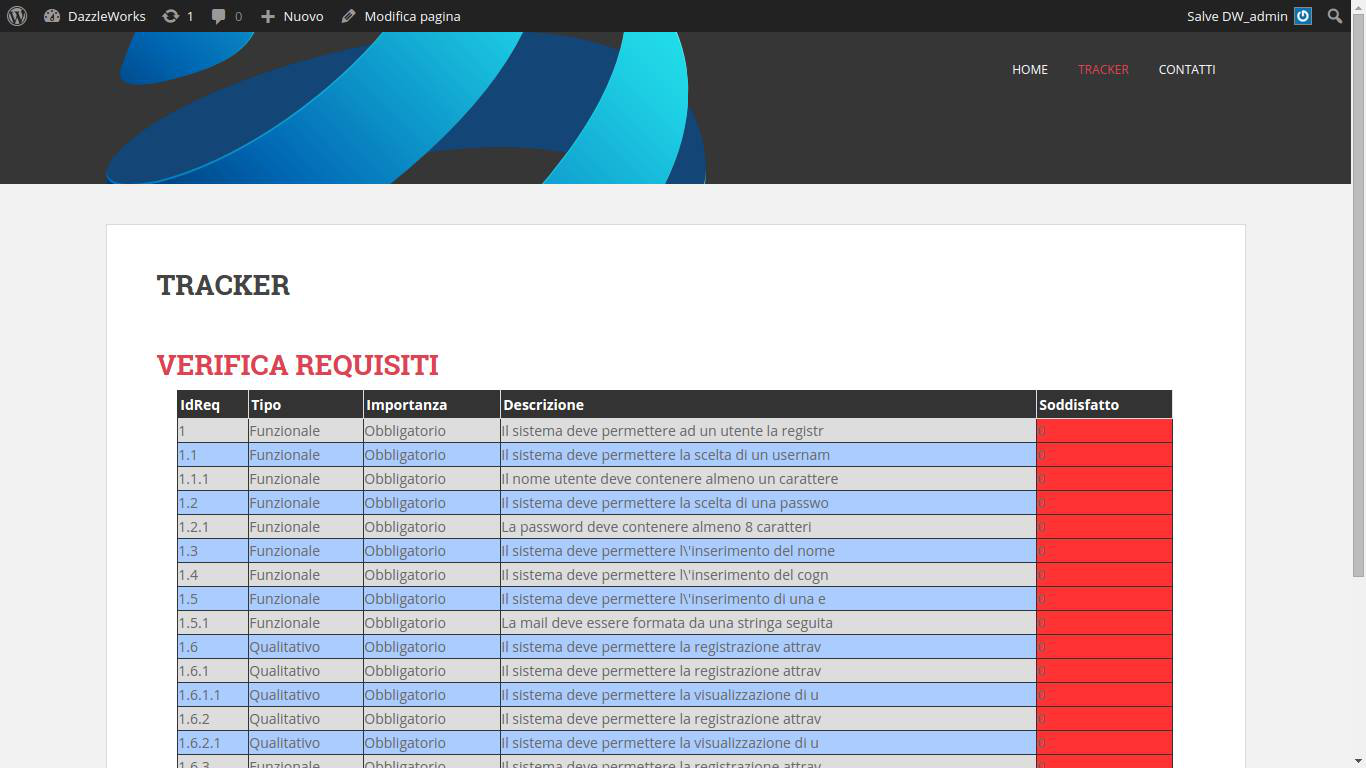
\includegraphics[width=0.7\linewidth]{img/tracker1}
	\caption[Pagina riepilogo requisiti]{Pagina riepilogo requisiti}
	\label{fig:tracker1}
	\end{figure}
	\begin{figure}[h]
		\centering
		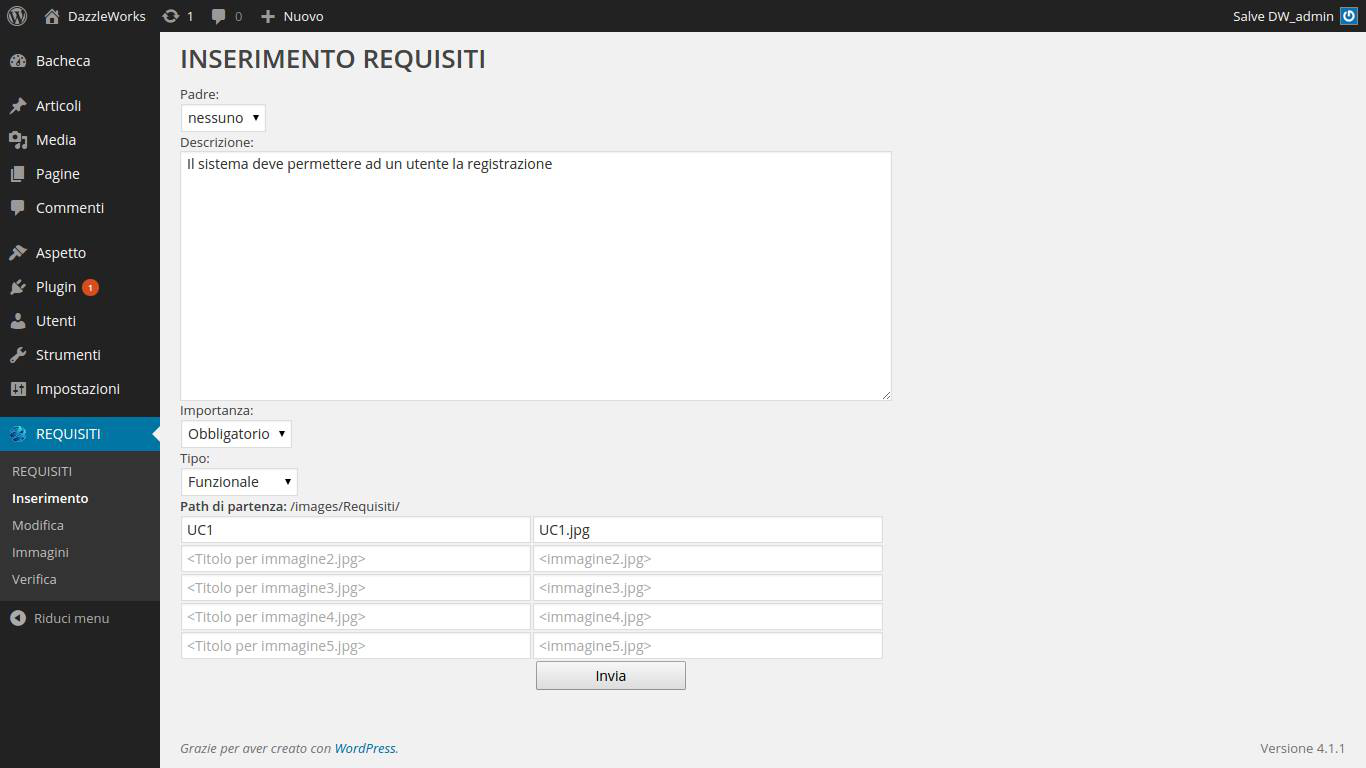
\includegraphics[width=0.7\linewidth]{img/tracker2}
		\caption[Pagina inserimento requisito]{Pagina inserimento requisito}
		\label{fig:tracker2}
		\end{figure}

\subsection{Progettazione}
Dopo la fase di \textbf{Analisi} si passerà alla fase di \textbf{Progettazione} dove i \textit{Progettisti} dovranno seguire le seguenti regole (organizzate per macro-aree).\\
\subsubsection{Specifica Tecnica}
I \textit{Progettisti} dovranno descrivere la progettazione ad alto livello dell'architettura del software e dei singoli componenti nella \textit{Specifica Tecnica}.

\paragraph{Diagrammi UML}
Dovranno essere realizzati i seguenti diagrammi:
\begin{itemize}
	\item Diagrammi delle classi;
	\item Diagrammi dei package;
	\item Diagrammi delle attività;
	\item Diagrammi di sequenza.
\end{itemize}
La lingua utilizzata nella realizzazione dei diagrammi sarà l'\textbf{inglese} e lo standard UML sarà 2.0.

\paragraph{Design Pattern}
I \textit{Progettisti} dovranno utilizzare il design pattern che ritengono più adatto al contesto per rendere l'applicazione più efficiente possibile. Ogni design pattern utilizzato verrà accompagnato da una breve descrizione e da un diagramma che ne esemplifica il funzionamento.

\paragraph{Classi di verifica}
Andranno create delle classi di verifica per testare che tutti i componenti abbiano un comportamento corretto.

\paragraph{Stile di progettazione}
Durante la fase di \textbf{Progettazione} bisognerà fare attenzione a:
\begin{itemize}
	\item \textbf{Ricorsione}: non dovrà essere utilizzata la ricorsione a meno che non sia strettamente necessaria. In quel caso dovrà essere fornita una dimostrazione induttiva sulla correttezza del metodo in questione;
	\item \textbf{Annidamento di cicli}: all'interno di un metodo non dovranno esserci cicli annidati con una profondità maggiore a cinque.
\end{itemize}

\subsection{Verifica}
La verifica dei processi, documenti e prodotti è un'attività da eseguire continuamente durante lo sviluppo del progetto. Di conseguenza, servono modalità operative chiare e dettagliate per i Verificatori, in modo da uniformare le attività di verifica svolte ed ottenere il miglior risultato possibile. Si descrivono ora le modalità ordinate e puntuali di verifica di processi, documenti, attività e codice alle quali ci si riferirà in questo documento e alle quali i Verificatori dovranno attenersi.

\subsubsection{Tecniche di analisi}
\paragraph{Walkthrough}
Cosiddetta lettura a pettine, questa tecnica di analisi prevede una lettura critica del codice o del documento prodotto. Tale tecnica è molto dispendiosa in termini di risorse, poiché viene applicata all'intero documento, senza avere una precisa idea di quale sia il tipo di anomalia e di dove ricercarla. Essa è però necessaria nelle prime fasi del progetto, vista l'inesperienza da parte del gruppo nell'attuare un tipo di verifica più precisa e mirata. Dopo una prima fase di lettura ed identificazione degli errori, si procede alla discussione degli stessi, proponendo le modifiche da apportare per garantirne la correzione. Il passo finale consiste nell'applicare le modifiche proposte, redigendo un rapporto preciso che elenchi le modifiche effettuate. Una caratteristica di questo tipo di analisi è che richiede l'utilizzo di più risorse umane;
\paragraph{Inspection}
Cosiddetta ricerca selettiva, questa tecnica di analisi presuppone l'esperienza da parte del verificatore nel individuare gli errori e le anomalie più frequenti. A tal scopo è necessaria una lista di controllo stilata in una precedente analisi di tipo walkthrough nella quale sono elencate le sezioni critiche. Questo ci consente una verifica più rapida e meno risorse umane. Dopo aver terminato l'analisi, è necessario stilare un rapporto di verifica.

\subsubsection{Verifica dei documenti}
La verifica dei documenti verrà eseguita ogni volta che è stata effettuata una modifica ad un documento e debba essere approvato.
Per una corretta verifica di un documento vanno seguite le seguenti pratiche:

\begin{itemize}
	\item \textbf{Controllo tipografico: }tramite l'utilizzo di TeXstudio verranno individuati errori tipografici presenti nel documento;
	\item \textbf{Controllo lessicale: }il \textit{Verificatore} dovrà controllore che il documento non presenti errori lessicali attraverso un'attenta analisi del testo utilizzando la tecnica \gls{inspection} o \gls{walkthrough};
	\item \textbf{Controllo glossario: }il \textit{Verificatore} dovrà controllore che ogni parola, nel testo, presente nel glossario sia correttamente evidenziata;
	\item \textbf{Controllo contenuto: }il \textit{Verificatore} dovrà controllare che il documento contenga tutto il necessario e che sia impaginato adeguatamente;
	\item \textbf{Rispetto delle norme del progetto: }il \textit{Verificatore} dovrà controllare che il documento segua le norme di progetto stabilite;
	\item \textbf{Lista di controllo: }si dovrà stilare una lista di errori più frequenti, per semplificare le successive verifiche dei documenti;
	\item \textbf{Rispetto \gls{indice Gulpease}: }il \textit{Verificatore} dovrà calcolare e controllare, per ogni documento, che gli \gls{indici di Gulpease} risiedano nel range di valori specificato nel \textit{Piano di Qualifica}, altrimenti si dovrà effettuare una ricerca \gls{walkthrough} alla ricerca delle frasi troppo lunghe e complesse;
	\item \textbf{Segnalazione errori: }una volta completata la verifica di un documento, se sono stati riscontrati errori, il \textit{Verificatore} dovrà aprire dei \gls{ticket} per segnalarli.
\end{itemize}
	
\subsubsection{Verifica dei diagrammi}
I diagrammi devono essere verificati manualmente dal \textit{Verificatore} e deve controllare che aderiscano correttamente allo standard \gls{UML} 2.0.
In particolare deve controllare che i diagrammi di flusso siano rappresentati in maniera corretta e che i \gls{casi d'uso} utilizzino correttamente le inclusioni e le estensioni.

\subsection{Codifica e Convenzioni}
\subsubsection{Linguaggi di codifica}
Dopo un'analisi del capitolato d'appalto e dei requisiti si è deciso che per lo sviluppo del software richiesto si utilizzeranno i linguaggi \gls{HTML5} , \gls{PHP} e \gls{Javascript}.

\subsubsection{Framework e librerie}
Per semplificare la realizzazione della nostra applicazione web si è deciso di utilizzare il \gls{framework} \gls{Angular}, per migliorare le interfacce utente, e la libreria \gls{Chart.js}, utilizzata per generare grafici.

\subsubsection{Convenzioni di codifica}
Di seguito è riportato l'insieme di norme e convenzioni che il gruppo dovrà seguire nella scrittura e documentazione del codice.
L'unica lingua ammessa per i nomi di variabili, metodi e commenti è l'inglese.

\subsubsection{File HTML}

Ogni file \gls{HTML} deve iniziare con il tag <!DOCTYPE html> che serve ad indicare che verrà utilizzata la versione \gls{HTML5}.
Ogni tag deve contenere un id e può contenere una o più classi.
Gli id e le classi dovranno essere contenute in un file .css a parte per mantenere il più possibile la separazione tra \gls{layout} e contenuto.
Le pagine \gls{HTML} devono rispettare gli standard del \gls{W3C}.

\subsubsection{Nomenclatura}
Per l'assegnazione di nomi a variabili, metodi e costanti andranno seguite le seguenti regole:
\begin{itemize}
	\item \textbf{Funzioni:} va utilizzata la notazione mixed case, con la prima lettera minuscola;
	\item \textbf{Variabili:} va utilizzata la notazione mixed case, con la prima lettera minuscola;
	\item \textbf{Costanti:} va scritto il nome interamente in maiuscolo, separando le varie parole con il carattere "\_" (underscore).
\end{itemize}

\subsubsection{Intestazione di un file Javascript}

\begin{flushleft}

/*\\
\vspace{3mm}
\begin{tabular}{l}
	File\\
	Autore\\
	Data\\
	Descrizione\\
\end{tabular}\\
\vspace{5mm}
 Modifiche:\\
 \vspace{3mm}
\begin{tabular}{| c c c c c c c c c |}
	\hline
	Versione & - & Data & - & Programmatore & - & Modifica & - & Descrizione\\
	\hline
	x.y.z & - & aaaa-mm-gg & - & Nome Cognome & - & Funzione & - & Descrizione modifica\\
	\hline
\end{tabular}\\
\vspace{3mm}
*/\\

\end{flushleft}

\begin{itemize}
	\item \textbf{File:} nome del file;
	\item \textbf{Autore:} nome e cognome del creatore del file;
	\item \textbf{Data:} data di creazione del file nel formato aaaa-mm-gg;
	\item \textbf{Descrizione:} poche righe di descrizione delle funzionalità contenute nel file;
	\item \textbf{Cambiamenti:} tabella dello stato di avanzamento del file, contenente tutte le modifiche effettuate :
		\begin{itemize}
			\item \textbf{Versione:} versione una volta effettuata la modifica;
			\item \textbf{Data:} data della modifica;
			\item \textbf{Programmatore:} nome e cognome del programmatore che ha effettuato la modifica;
			\item \textbf{Modifica:} segnatura della funzione a cui è stata apportata una modifica;
			\item \textbf{Descrizione:} breve descrizione della modifica effettuata.
		\end{itemize}
\end{itemize}

\subsubsection{Commenti}

Prima di ogni funzione dovrà essere presente un commento con la seguente forma:

\begin{flushleft}
/*\\
\vspace{3mm}
\begin{tabular}{l}
	Descrizione della funzione\\
	Descrizione dei parametri\\		
	Descrizione del tipo di ritorno\\
\end{tabular}\\
\vspace{3mm}
*/

\end{flushleft}

Ogni variabile di particolare importanza dovrà essere fornita di commento che ne spieghi scopo e funzionamento.

